\documentclass{article}
\usepackage{natbib}
\usepackage{graphicx}
\usepackage{csquotes}
\usepackage{hyperref}
\usepackage{booktabs}
\usepackage{multirow}
\usepackage[table]{xcolor} 
\usepackage{graphicx}
\usepackage{caption}
\usepackage{amsmath}
\usepackage{rotating}
\usepackage{wrapfig}
\usepackage[margin=4cm]{geometry}

%---------------------------------- NATBIB ----------------------------------%
\makeatletter
% natbib: only make year a hyperref, not author
\let\oldciteauthor\citeauthor

\def\citeauthor#1{{\NoHyper\oldciteauthor{#1}}}

% Patch case where name and year are separated by aysep
\patchcmd{\NAT@citex}
  {\@citea\NAT@hyper@{%
     \NAT@nmfmt{\NAT@nm}%
     \hyper@natlinkbreak{\NAT@aysep\NAT@spacechar}{\@citeb\@extra@b@citeb}%
     \NAT@date}}
  {\@citea\NAT@nmfmt{\NAT@nm}%
   \NAT@aysep\NAT@spacechar\NAT@hyper@{\NAT@date}}{}{}

% Patch case where name and year are separated by opening bracket
\patchcmd{\NAT@citex}
  {\@citea\NAT@hyper@{%
     \NAT@nmfmt{\NAT@nm}%
     \hyper@natlinkbreak{\NAT@spacechar\NAT@@open\if*#1*\else#1\NAT@spacechar\fi}%
       {\@citeb\@extra@b@citeb}%
     \NAT@date}}
  {\@citea\NAT@nmfmt{\NAT@nm}%
   \NAT@spacechar\NAT@@open\if*#1*\else#1\NAT@spacechar\fi\NAT@hyper@{\NAT@date}}
  {}{}
  
\makeatother
%-------------------------------------------------------------------------------%


%----------------------------------- HREF ------------------------------------%
% define href colors
\hypersetup{
    colorlinks=true,
    linkcolor=blue,
    filecolor=blue,      
    urlcolor=blue,
    citecolor=blue
}
\urlstyle{same}
%-------------------------------------------------------------------------------%


\begin{document}
\graphicspath{ {../../../output/03-results/plots/} }

\section{Analyzing Legal Language Using Corpus Analysis}

\subsection{Selecting Terms of Interest}

The data for this study comprises two distinct corpora: a corpus with legal documents and a corpus with comments from Reddit, the world's largest online-forum. The legal corpus (LC) contains court opinions from Court of Appeals for the 1st to 11th regional circuit (without DC and the federal court), based on open data provided by the \citet{FreeLawProject2020}.\footnote{The Court of Appeals are the intermediate appellate courts of the United States federal judiciary. Each of the so-called regional circuits hears appeals from the district courts within its borders, or from other designated federal courts and administrative agencies. The appeals from the circuit courts are taken to the Supreme Court of the United States, which means that circuit court decisions are quite influential. Moreover, circuit court decisions, establish binding precedents, unlike those of the lower federal courts. The lower federal courts have to follow the guidance of their circuit court in similar cases, irrespective of the trial judge's opinion.} For the Reddit corpus (RC), we gathered data using the API for the Pushshift Reddit Data Set provided by \citet{Baumgartner2020}. 

In our case, the corpus generation is an iterative process. We start off with a list of target adjectives we specified without information about the corpora, and are based on the literature. This initial list contains adjectives in two categories, namely descriptive concepts or concepts which have a high potential to count as thick concepts. Among those thick concepts, we created sub-groups which differ in what non-descriptive information might be conveyed. First, there are ethical thick concepts whose non-descriptive content is ethical in nature. Examples were selected based on the vast literature on thick ethical concepts that are of special interest in the legal domain, as offences in the criminal law are not merely legal offences, but transgress moral norms too. Second, the legal system operates within a set of epistemic norms -- norms of what we should believe and may conclude from a given set of premises. We therefore created a group of thick epistemic concepts which is inspired by the philosophical literature. Finally, it is plausible to believe that some thick concepts are used exclusively or predominantly in the legal context, such as the term \enquote{legal} itself. 
%This initial list contains  adjectives that often discussed by the TC-literature, as well as descriptive, epistemic, and legal concepts. However, it turns out that some of these adjectives are rarely used in the legal context, while others may occur frequently, yet are most often part of legal phrases, which indicate a different semantic embedding. In order to avoid selection bias and exclude adjectives with predominantly phrasal use, we inductively select a second battery of adjectives that is used complementary to the first. 

However, it turns out that some of these adjectives are rarely used in the legal context, while others may occur frequently, yet are most often part of legal phrases, which indicate a different semantic embedding. In order to avoid selection bias and exclude adjectives with predominantly phrasal use, we inductively select a second battery of adjectives that is used complementary to the first. This inductive approach is based on an analysis of part of speech (PoS)-sequences in the legal corpus. PoS-tagging is an unsupervised method to annotate the syntactic structure of text data. For each of the subcorpora (1st to 11th Court of Appeals), we first draw a random sample of 2000 documents which are subsequently PoS-tagged using UDPipe \citep{Straka2017, Straka2020}. Based on these PoS-tags, we isolate all syntactic structures of the form $(M)*A(,)*C(M)*A$ (M = modifier, A = adjective, C = conjunction, (...) = optional part). Finally, all adjectives are ranked according to frequency as well lexical diversity in regards to the conjoined adjectives. We use Yule's \textit{K} \citep{Yule1944, Tweedie1998} as a measure for lexical diversity.  %In addition, we map them on a dissociation dimension, which gives a measure of how exclusive the set of conjoined adjectives is for a specific $A_i$.
Based on this ranking, we manually select adjectives that match our concept classes and retrieve documents containing suitable target structures both from the legal corpus and via the Pushshift API. % In a last step, we determine the three most promising concepts per class, based on number of occurences and Yule's $K$, and reduce the respective corpora accordingly. 
The final list of 24 adjectives is shown in Table \ref{tab:ADJlist} below.

\begin{table}[!h]
\centering
\rotatebox{90}{%
\begin{minipage}{\textwidth}
\normalsize
\rowcolors{5}{gray!25}{white}
\begin{tabular}{lllrrrrrrrr}
  & & & \multicolumn{3}{c}{Sentiment Quantiles} & & & \multicolumn{3}{c}{Lex. Diversity}\\
  \cmidrule{4-6} \cmidrule{9-11}
  Class & Target & Polarity & 25\% & 50\% & 75\% & Avg. & N &  TTR & CTTR & K\\
  \bottomrule
Descriptive & active & neutral & -0.10 & 0.08 & 0.27 & 0.07 & 948 & 0.21 & 4.64 & 343.83 \\ 
  Descriptive & ambiguous & neutral & -0.35 & -0.18 & -0.03 & -0.19 & 1182 & 0.16 & 3.93 & 638.53 \\ 
  Descriptive & complex & neutral & -0.16 & 0.00 & 0.16 & -0.01 & 1954 & 0.14 & 4.26 & 292.63 \\ 
  Descriptive & explicit & neutral & 0.03 & 0.21 & 0.23 & 0.13 & 1565 & 0.11 & 3.18 & 982.63 \\ 
  Descriptive & limited & neutral & -0.01 & 0.08 & 0.23 & 0.09 & 1501 & 0.19 & 5.27 & 375.77 \\ 
  Descriptive & practical & neutral & 0.01 & 0.19 & 0.29 & 0.18 & 1338 & 0.13 & 3.31 & 444.01 \\ 
  Epistemic & illogical & negative & -0.50 & -0.39 & -0.20 & -0.33 & 3855 & 0.16 & 7.13 & 143.74 \\ 
  Epistemic & inappropriate & negative & -0.57 & -0.45 & -0.27 & -0.39 & 6161 & 0.11 & 6.04 & 152.70 \\ 
  Epistemic & inconsistent & negative & -0.45 & -0.34 & -0.05 & -0.26 & 4847 & 0.16 & 7.98 & 100.21 \\ 
  Epistemic & consistent & positive & 0.06 & 0.24 & 0.50 & 0.26 & 7038 & 0.13 & 7.59 & 117.42 \\ 
  Epistemic & logical & positive & 0.17 & 0.27 & 0.41 & 0.28 & 8426 & 0.10 & 6.44 & 201.46 \\ 
  Epistemic & reasonable & positive & 0.06 & 0.18 & 0.35 & 0.22 & 15523 & 0.05 & 4.47 & 260.49 \\ 
  Legal & illegal & negative & -0.55 & -0.42 & -0.11 & -0.34 & 3633 & 0.15 & 6.41 & 269.85 \\ 
  Legal & unjust & negative & -0.55 & -0.42 & -0.27 & -0.37 & 2879 & 0.15 & 5.53 & 234.55 \\ 
  Legal & unlawful & negative & -0.42 & -0.17 & 0.11 & -0.15 & 1566 & 0.17 & 4.75 & 235.22 \\ 
  Legal & lawful & positive & -0.08 & 0.19 & 0.50 & 0.16 & 1699 & 0.14 & 4.15 & 427.35 \\ 
  Legal & legal & positive & 0.01 & 0.22 & 0.22 & 0.18 & 14254 & 0.04 & 3.70 & 1189.78 \\ 
  Legal & legitimate & positive & 0.00 & 0.24 & 0.41 & 0.20 & 6539 & 0.10 & 5.91 & 252.86 \\ 
  TC & dishonest & negative & -0.55 & -0.45 & -0.34 & -0.40 & 5271 & 0.13 & 6.63 & 122.17 \\ 
  TC & improper & negative & -0.44 & -0.42 & -0.12 & -0.30 & 1906 & 0.17 & 5.38 & 521.61 \\ 
  TC & unfair & negative & -0.51 & -0.39 & -0.27 & -0.36 & 7617 & 0.10 & 5.95 & 175.56 \\ 
  TC & careful & positive & 0.06 & 0.29 & 0.46 & 0.26 & 4200 & 0.12 & 5.30 & 211.82 \\ 
  TC & honest & positive & 0.21 & 0.32 & 0.51 & 0.32 & 6624 & 0.09 & 5.21 & 356.66 \\ 
  TC & proper & positive & 0.06 & 0.22 & 0.45 & 0.23 & 7884 & 0.10 & 6.01 & 424.46 \\ 
   \hline
\end{tabular}
\end{minipage}
}
\caption{Final Adjective List}
\label{tab:ADJlist}
\end{table}


\subsection{The Data}

%\subsection{Method}
%In the following, we will discuss the methods used in our two studies.

The full LC has 49'199 entries, whereas RC has 69'211. Both corpora are cleaned, PoS-tagged, lemmatized and the conjoined adjectives are annotated with sentiment values from the SentiWords dictionary based on SENTIWORDNET \citep{Esuli2006, Baccianella2010, Guerini2013, Gatti2016}. In the following we present the summary statistics for each corpus. Table \ref{tab:LCstats} shows the measures of sentiment dispersion and lexical diversity by class and polarity for LC. Table \ref{tab:BCstats} contains the same for RC. 

The sentiment dispersion in Table \ref{tab:LCstats} indicates more extreme values for negative target adjectives overall. According to Yule's \textit{K}, their conjuncts are also more lexically diverse than the ones of the positive target adjectives. The average observed sentiment is consistent with our assumption that AND-conjunctions pair adjectives of the same polarity. Descriptive concepts have a very neutral average (0.05), which is also consistent with our expectations. However, there seems to be an overlap between descriptive concepts and of the several concept classes, which might prove to be significant later on.

\begin{table}[!h]
\centering
\rowcolors{5}{gray!25}{white}
\begin{tabular}{rlrrrrrrrr}
  & & \multicolumn{3}{c}{Sentiment Quantiles} & & \multicolumn{3}{c}{Lex. Diversity}\\
   \cmidrule{3-5} \cmidrule{7-9}
  Class & Polarity & 25\% & 50\% & 75\% & Avg. &  TTR & CTTR & K\\
  \bottomrule
Descriptive & neutral & -0.08 & 0.03 & 0.23 & 0.05 & 0.11 & 6.98 & 102.40 \\ 
%Descriptive & negative & -0.03 & 0.06 & 0.23 & 0.06  & 0.12 & 6.02 & 192.24 \\ 
  %Descriptive & positive & -0.18 & 0.00 & 0.22 & 0.02  & 0.15 & 6.17 & 168.36 \\ 
  Epistemic & negative & -0.44 & -0.33 & -0.10 & -0.26 & 0.16 & 6.09 & 124.78 \\ 
  Epistemic & positive & 0.04 & 0.14 & 0.30 & 0.17 & 0.05 & 3.68 & 342.11 \\ 
  Legal & negative & -0.40 & -0.29 & 0.00 & -0.19 & 0.13 & 4.69 & 249.80 \\ 
  Legal & positive & 0.07 & 0.22 & 0.22 & 0.17 & 0.04 & 2.93 & 1530.47 \\ 
  TC & negative & -0.44 & -0.35 & -0.20 & -0.30 & 0.11 & 4.81 & 507.77 \\ 
  TC & positive & 0.06 & 0.16 & 0.33 & 0.21 & 0.06 & 3.55 & 640.33 \\ 
   \hline
\end{tabular}
\caption{Summary Statistics LC}
\label{tab:LCstats}
\end{table}

Table \ref{tab:RCstats} indicates a far more polar sentiment dispersion in RC compared to LC, which is also reflected by the more polar averages. Lexical diversity is a lot higher in RC than LC, which was to be expected, due to the more codified nature of legal language use. The difference in homogeneity is most acute for legal concepts and TC, but less so for epistemic concepts.

\begin{table}[!h]
\centering
\rowcolors{5}{gray!25}{white}
\begin{tabular}{rlrrrrrrrr}
  & & \multicolumn{3}{c}{Sentiment Quantiles} & & \multicolumn{3}{c}{Lex. Diversity}\\
   \cmidrule{3-5} \cmidrule{7-9}
  Class & Polarity & 25\% & 50\% & 75\% & Avg. &  TTR & CTTR & K\\
  \bottomrule
Epistemic & negative & -0.52 & -0.42 & -0.18 & -0.34 & 0.10 & 7.65 & 73.19 \\ 
  Epistemic & positive & 0.16 & 0.29 & 0.50 & 0.30 & 0.08 & 7.26 & 94.69 \\ 
  Legal & negative & -0.55 & -0.44 & -0.24 & -0.38 & 0.13 & 6.65 & 198.62 \\ 
  Legal & positive & 0.00 & 0.22 & 0.45 & 0.21 & 0.09 & 6.43 & 132.81 \\ 
  TC & negative & -0.55 & -0.45 & -0.29 & -0.39 & 0.09 & 6.93 & 80.10 \\ 
  TC & positive & 0.16 & 0.32 & 0.52 & 0.31 & 0.09 & 7.06 & 125.27 \\ 
   \hline
\end{tabular}
   \caption{Summary Statistics RC}
   \label{tab:BCstats}
\end{table}

The sentiment dispersion on the level of the target adjectives shared by LC and RC are shown in Figure \ref{fig:SDta}. As we can see, the polarity of the target adjective is a good indicator for the polarity of the conjoined adjective, and vice versa. With the exception of \textit{lawful} and \textit{unlawful}, the sentiment spread is mostly limited to either the positive or the negative region of the scale and does not include the midpoint. The differences between the corpora we noted above are also present on the level of the target adjectives: LC has lower averages (i.e. dots) than BC across the board, with the exception of \textit{dishonest} and \textit{improper}. %This becomes even more apparent on when aggregated by class (i.e. horizontal lines).

\begin{figure}[!ht]
\center
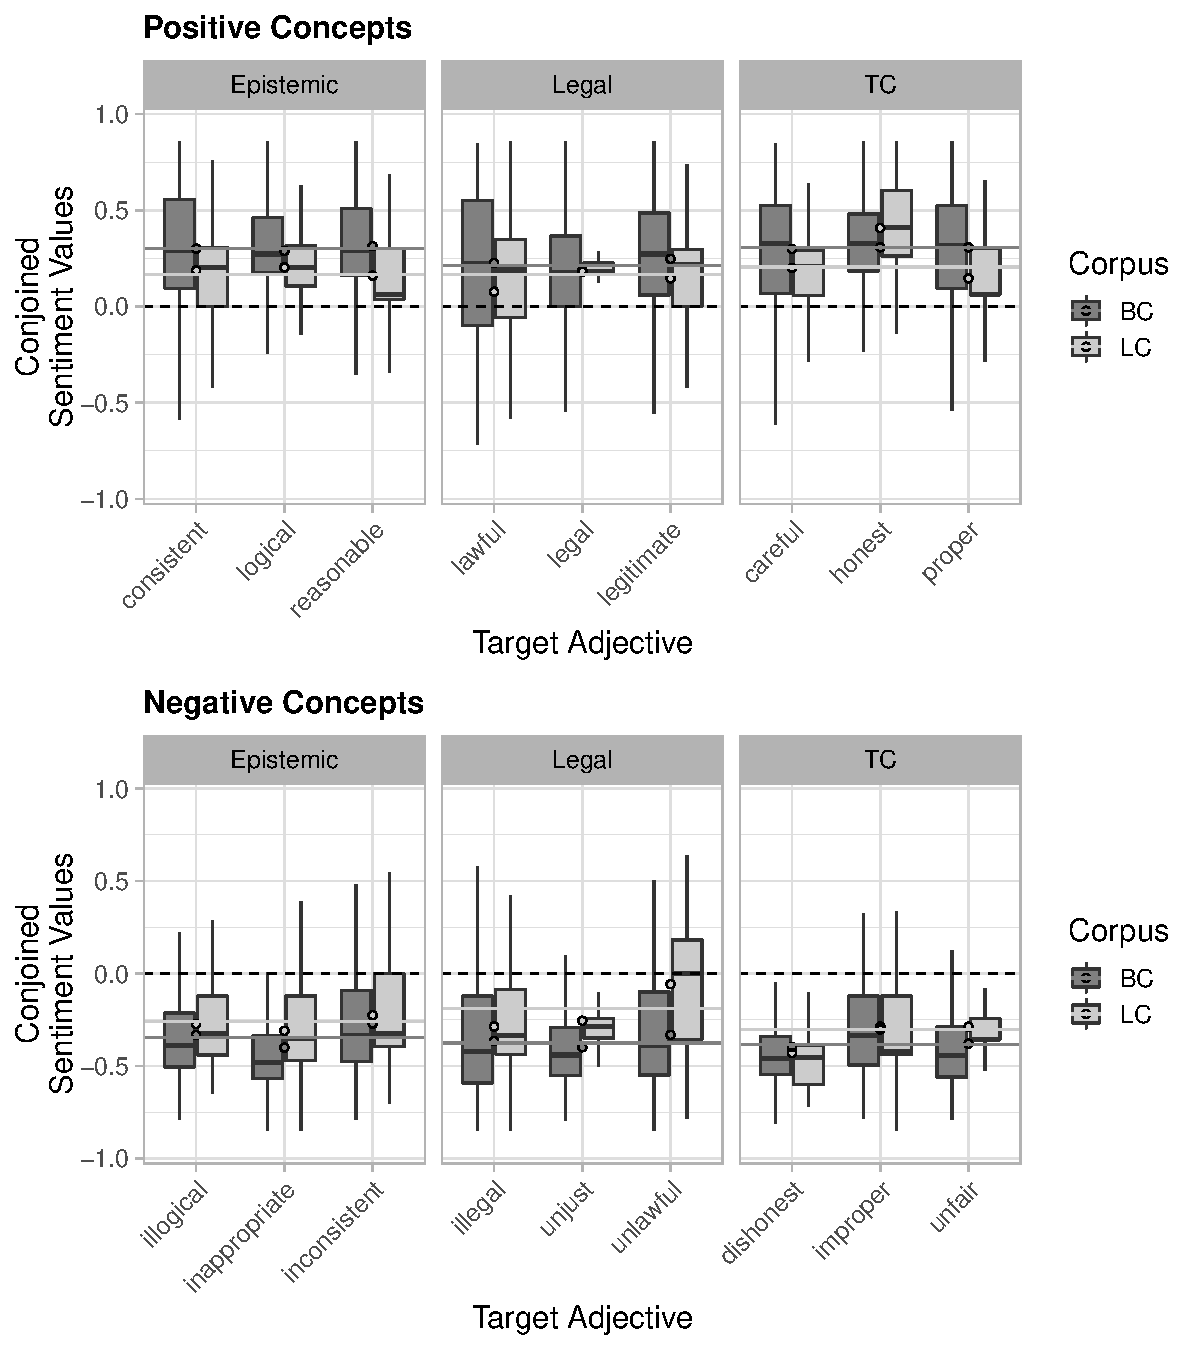
\includegraphics[width=.9\textwidth, keepaspectratio]{bc_lc_summary_stats_adj-distr}
\caption{Sentiment Dispersion by Target Adjective}
\label{fig:SDta}
\end{figure}


\subsection{Study 1}

%\subsubsection{Hypotheses and Method}
\subsection{Proceeding}

In the first study, we assess the average context effects for both corpora. First, we estimate the average sentiment intensity of conjoined adjectives in each corpus. The basis for this analysis is a linear model with the absolute conjoined sentiment values as dependent and the corpus-dummy as independent variable. Based on this model, we compute the estimated marginal means for the corpora. This gives on overall estimate of differences in sentiment intensity between the corpora, irrespective of polarity. 

In the first study, we assess the average context effects for both corpora. The first hypothesis concerns the average absolute sentiment intensity of conjoined adjectives in each corpus: we expect the legal corpus to contain conjunctions with more neutral sentiment values than the Reddit corpus ($H_1$). In order to test $H_1$, we use a linear model with the absolute conjoined sentiment values as dependent variable and the corpus-dummy (RC/LC) as independent variable. Based on this model, we compute the estimated marginal means (EMM) for the corpora. This gives us an overall estimate of differences in sentiment intensity between the corpora, irrespective of sentiment polarity (pos/neg). 

The second model further discriminates between positive and negative target adjectives, but does not yet include the concept classes. Instead of using absolute sentiment values as dependent variable, this model uses the non-transformed values. The polarity-discriminator is added as an interaction term between the corpus-dummy and the polarity-dummy for the target adjectives. This allows us to assess the estimated marginal means of the conjoined sentiment values for each corpus by target polarity.

For the second hypothesis, we further discriminate between positive and negative target adjectives%, but does not yet include the concept classes
. As with $H_1$, we expect the legal corpus to have more neutral conjoined sentiment values on average, and that the effect is significant for both positive and negative target adjectives ($H_2$). On the one hand, $H_{2a}$ posits that conjoined sentiment values for negative target adjectives are on average significantly closer to 0 in the case of the legal corpus compared to the Reddit corpus.  On the other hand, $H_{2b}$ assumes the same for positive target adjectives. In contrast to $H_1$ we are not only interested in sentiment intensity, but also also in polarity. Thus the second model uses the non-transformed sentiment values as dependent variable, instead of absolute sentiment values used to test $H_1$. The polarity-discriminator (pos/neg) is added as an interaction term between the corpus-dummy and the polarity-dummy for the target adjectives. This allows us to assess the estimated marginal means of the conjoined sentiment values for each corpus by target polarity.


The third and final model estimates the differences between corpora for each concept class. Because we are mostly interested in differences in terms of intensity, the model once again uses absolute conjoined sentiment values. As estimator we use an interaction term between the corpus dummy and the concept class factor.

The third and final model hypothesis is that the difference between the corpora further persist across all concept classes. We expect more neutral average sentiment values for each concept class in the legal corpus compared to the same concept class in the Reddit corpus ($H_3$). Because we are mostly interested in differences in terms of intensity, the third model once again uses absolute conjoined sentiment values, as for testing for $H_1$. As estimator we use an interaction term between the corpus dummy (BC/LC) and the concept class factor (Epistemic/Legal/TC). The partial hypotheses are defined as follows: $H_{3a}$ assumes that epistemic concepts have lower average conjoined sentiment values in LC compared to BC. $H_{3b}$ expects that the same holds for legal concepts, while $H_{3c}$ does so for TC.



\subsubsection{Results}

The first model of study 1 is presented in Table \ref{tab:s1m1} and shows the effect of context (LC v. RC) on the absolute sentiment of conjoined adjectives. According to the linear model, LC has an average effect of $\beta = -0.1262$ compared to RC, $t\text{-value:} -99.63$, $Pr(>|t|) = <2e^{-16}$, all other things equal. The estimated marginal mean for RC is $0.3622$, the one for LC is $0.2360$. Hence, the sentiment values of the conjoined adjectives are indeed less intense for LC than for RC.

\begin{table}[!h]
\centering
\begin{tabular}{lrrrrr}
  \hline
Corpus & Est. Mean & SE & df & lower CL & upper CL \\ 
  \hline
RC & 0.3622 & 0.0008 & 109920 & 0.3607 & 0.3637 \\ 
  LC & 0.2360 & 0.0010 & 109920 & 0.2341 & 0.2380 \\ 
   \hline
\multicolumn{6}{l}{{\footnotesize Results are given on the absolute scale. Confidence level used: 0.95}}\\
\end{tabular}
\caption{Absolute Estimated Mean Sentiment Difference Between Corpora}
\label{tab:s1m1}
\end{table}

The second model shows similar results, even if we take polarity into account. The effect of positive polarity compared to negative polarity is $\beta_1 = 0.6456$, $t\text{-value:}\ 324.43$, whereas the effect of LC compared to RC drops slightly to $\beta_2 = 0.1085$, $t\text{-value:}\ 35.31$. The interaction of positive polarity and LC compared to the intercept has an effect of $\beta_3 = -0.2130$, $t\text{-value:}-58.68$. All effects are highly significant on a 0.05 alpha-level ($Pr(>|t|) = <2e^{-16}$). Table \ref{tab:s1m2} contains the estimated marginal means for this model. In summary, LC has significantly more neutral sentiment values than RC on both sides of the sentiment scale.

\begin{table}[!h]
\centering
\begin{tabular}{lrrrrr}
  \hline
Corpus & Est. Mean & SE & df & lower CL & upper CL \\ 
\hline
\multicolumn{6}{l}{Polarity = negative}\\
\cmidrule{1-2}
RC & -0.3659 & 0.0015 & 109918 & -0.3689 & -0.3629 \\ 
  LC & -0.2574 & 0.0027 & 109918 & -0.2627 & -0.2522 \\ 
   \cmidrule{1-6}
\multicolumn{6}{l}{Polarity = positive}\\
\cmidrule{1-2}
RC & 0.2797 & 0.0013 & 109918 & 0.2772 & 0.2822 \\ 
  LC & 0.1752 & 0.0015 & 109918 & 0.1723 & 0.1780 \\ 
   \hline
\multicolumn{6}{l}{{\footnotesize Confidence level used: 0.95}}\\
\end{tabular}
\caption{Estimated Mean Difference Between Corpora by Target Polarity}
\label{tab:s1m2}
\end{table}

Table \ref{tab:s1m3} shows the contrasts between the absolute estimates for each concept class and corpus. The differences indicate higher estimated values for RC compared to LC across the board, which is consistent with the findings of the previous models. Interestingly, legal concepts show the smallest difference of all concept classes. All contrasts are significant on a 0.05 alpha-level. The effect sizes for all estimators can be found in Table \ref{tab:s1m3lm} in the \hyperref[sec:appendix]{Appendix}. This shows that the differences between legal and everyday use of concepts are robust across concept classes.

\begin{table}[ht]
\centering
\begin{tabular}{lrrrrl}
  \hline
Contrast & Estimate & SE & df & $t$-ratio & $p$-value \\ 
  \hline
\multicolumn{6}{l}{Class = Epistemic}\\
RC - LC & 0.1426 & 0.0020 & 109916 & 71.640 & $<$.0001 \\ 
\cmidrule{1-1}
\multicolumn{6}{l}{Class = Legal}\\
RC - LC & 0.0985 & 0.0023 & 109916 & 42.669 & $<$.0001 \\ 
\cmidrule{1-1}
\multicolumn{6}{l}{Class = TC}\\
RC - LC & 0.1153 & 0.0024 & 109916 & 48.231 & $<$.0001 \\ 
   \hline
\multicolumn{6}{l}{{\footnotesize Note: contrasts are still on the abs scale}}\\
\end{tabular}
\caption{Planned Absolute Contrasts by Concept Class}
\label{tab:s1m3}
\end{table}

\iffalse
\begin{table}[ht]
\centering
\begin{tabular}{lrrrrl}
  \hline
Contrast & Estimate & SE & df & $t$-ratio & $p$-value \\ 
  \hline
\multicolumn{6}{l}{Corpus = RC}\\
\cmidrule{1-1}
\rowcolor{gray!25} Epistemic - Legal & 0.0314 & 0.0020 & 109916 & 15.798 & $<$.0001 \\  Epistemic - TC & -0.0261 & 0.0018 & 109916 & -14.854 & $<$.0001 \\ 
\rowcolor{gray!25}  Legal - TC & -0.0575 & 0.0021 & 109916 & -27.550 & $<$.0001 \\ 
   \midrule
\multicolumn{6}{l}{Corpus = LC}\\
\cmidrule{1-1}
\rowcolor{gray!25} Epistemic - Legal & -0.0128 & 0.0023 & 109916 & -5.530 & $<$.0001 \\ 
  Epistemic - TC & -0.0534 & 0.0026 & 109916 & -20.791 & $<$.0001 \\ 
 \rowcolor{gray!25} Legal - TC & -0.0406 & 0.0026 & 109916 & -15.699 & $<$.0001 \\ 
   \hline
\multicolumn{6}{l}{{\footnotesize Note: contrasts are still on the absolute scale. Confidence level used: 0.95}}\\
\multicolumn{6}{l}{{\footnotesize P value adjustment: tukey method for comparing a family of 3 estimates}}\\
\end{tabular}
\caption{Planned Absolute Contrasts by Corpus}
\end{table}
\fi


\subsection{Study 2}

%\subsubsection{Hypotheses and Method}
\subsection{Proceeding}

In the second study, we focus on the legal corpus only. In order to be able to compare the results of the evaluative concepts classes to a baseline, we added corpus entries for the following descriptive target adjectives: \textit{active}, \textit{ambiguous}, \textit{complex}, \textit{explicit}, \textit{limited}, and \textit{practical}. Instead of comparing context effects (Study 1), we want to inquire whether the concept classes can be distinguished from each other within the legal context. The linear model includes the absolute conjoined sentiment as dependent variable and the concept classes as independent variable, followed by pairwise contrasts between the estimated marginal means of the concept classes. This will allow us to asses differences in sentiment intensity. 
%The second model further discriminates between the polarity of the target adjectives. 
We cannot perform planned contrasts by target polarity, because the descriptive concept only have a neutral polarity, which leads to empty interaction levels and contrasts. %The second model includes and interaction term of polarity and concept class and uses non-transformed sentiment values, in order to measure polarity-differences along the sentiment scale between the classes. %cluster differently within the legal context. We use a combination of K-Means Clustering and Principal Component Analysis (PCA), which is informed by the sentiment values of the conjoined adjectives and a measure for lexical diversity of the target adjective, i.e. Yule's \textit{K} \citep{Yule1944, Tweedie1998}. The cluster analysis further includes information based on the vector space of the corpus, which is created using the \textit{Semantic Vectors} package \citep{Widdows2008, Widdows2010, Widdows2016}. For every pair of target adjective and conjoined adjective, we compute the cosine similarities. Cosine similarities are essentially high dimensional representations of co-occurence measures, and inform the cluster analysis about the semantic similarity of the conjuncts by taking the whole corpus into account. In the final ANOVA model, the cosine similarities are added as weights for the sentiment values of the conjoined adjectives.

%\section{Results}

%Before we move to the results of our studies, there will be a brief discussion of the summary statistics of the text data.

%\subsection{Study 1}

\subsubsection{Results}

In study 2, we focus on LC and add descriptive concepts as a baseline. The aim of this study is to assess the possibility of distinguishing concept classes within the legal discourse, based on sentiment values. Table \ref{tab:s2m1} presents the absolute contrasts between the concept classes in LC. As we can see, all concept classes have significantly different sentiment intensity (0.05 alpha-level), which indicates, that a there is no need to further discriminate by polarity in order to distinguish the classes from each other. The smallest differences are between epistemic and legal concepts ($\Delta\bar{y}=-0.0128$), descriptive and epistemic concepts ($\Delta\bar{y}=-0.0140$), as well as descriptive and legal concepts ($\Delta\bar{y}=-0.0268$). The contrasts involving TC, on the other hand, have a much wider spread. %As we can see, the newly introduced baseline does not have a significantly different sentiment intensity compared to legal concepts ($\Delta\bar{y}=-0.0027$, $p$-value: 0.8548), on a 0.05 alpha-level. All the other contrasts are significant. %Hence, in regards to our cluster analysis, we can expect the different target adjectives from the same concept class to cluster together, with the exception of descriptive concepts, which might overlap with epistemic concepts.
%This means that legal concepts are used in conjunction with adjectives that do have a similar sentiment intensity to the ones of descriptive concepts.

\begin{table}[ht]
\centering
\begin{tabular}{lrrrrl}
  \hline
Contrast & Estimate & SE & df & $t$-ratio & $p$-value \\ 
  \hline
\rowcolor{gray!25}Desc. - Epistemic & -0.0140 & 0.0024 & 49195 & -5.873 & $<$.0001 \\ 
  Desc. - Legal & -0.0268 & 0.0024 & 49195 & -11.147 & $<$.0001 \\ 
 \rowcolor{gray!25} Desc. - TC & -0.0674 & 0.0026 & 49195 & -25.942 & $<$.0001 \\ 
  Epistemic - Legal & -0.0128 & 0.0020 & 49195 & -6.298 & $<$.0001 \\ 
 \rowcolor{gray!25} Epistemic - TC & -0.0534 & 0.0023 & 49195 & -23.678 & $<$.0001 \\ 
  Legal - TC & -0.0406 & 0.0023 & 49195 & -17.880 & $<$.0001 \\ 
   \hline
\multicolumn{6}{l}{{\footnotesize Note: contrasts are still on the abs scale}}\\

\multicolumn{6}{l}{{\footnotesize P value adjustment: tukey method for comparing a family of 4 estimates}}\\
\end{tabular}
\label{tab:s2m1}
\end{table}

\iffalse
\begin{table}[ht]
\centering
\begin{tabular}{lrrrrl}
  \hline
Contrast & Estimate & SE & df & $t$-ratio & $p$-value \\ 
  \hline
\rowcolor{gray!25}Desc. - Epistemic & 0.0101 & 0.0034 & 44175 & 3.013 & 0.0138 \\ 
  Desc. - Legal & -0.0027 & 0.0034 & 44175 & -0.799 & 0.8548 \\ 
\rowcolor{gray!25}  Desc. - TC & -0.0433 & 0.0035 & 44175 & -12.355 & $<$.0001 \\ 
  Epistemic - Legal & -0.0128 & 0.0020 & 44175 & -6.253 & $<$.0001 \\ 
\rowcolor{gray!25}  Epistemic - TC & -0.0534 & 0.0023 & 44175 & -23.510 & $<$.0001 \\ 
  Legal - TC & -0.0406 & 0.0023 & 44175 & -17.752 & $<$.0001 \\ 
   \hline
\multicolumn{6}{l}{{\footnotesize Note: contrasts are still on the absolute scale. Confidence level used: 0.95}}\\
\multicolumn{6}{l}{{\footnotesize P value adjustment: tukey method for comparing a family of 4 estimates}}\\
\end{tabular}
\caption{Planned Absolute Contrasts by Class}
\label{tab:s2m1}
\end{table}


\begin{table}[ht]
\centering
\begin{tabular}{lrrrrl}
  \hline
Contrast & Estimate & SE & df & $t$-ratio & $p$-value \\ 
  \hline
\multicolumn{6}{l}{Polarity = negative}\\
\cmidrule{1-1}
\rowcolor{gray!25}Desc. - Epistemic & 0.3227 & 0.0054 & 49191 & 60.098 & $<$.0001 \\ 
  Desc. - Legal & 0.2516 & 0.0055 & 49191 & 45.702 & $<$.0001 \\ 
 \rowcolor{gray!25} Desc. - TC & 0.3647 & 0.0049 & 49191 & 75.186 & $<$.0001 \\ 
  Epistemic - Legal & -0.0712 & 0.0062 & 49191 & -11.474 & $<$.0001 \\ 
 \rowcolor{gray!25} Epistemic - TC & 0.0420 & 0.0056 & 49191 & 7.458 & $<$.0001 \\ 
  Legal - TC & 0.1132 & 0.0058 & 49191 & 19.650 & $<$.0001 \\ 
   \midrule
\multicolumn{6}{l}{Polarity = positive}\\
\cmidrule{1-1}
\rowcolor{gray!25}Desc. - Epistemic & -0.1456 & 0.0044 & 49191 & -33.374 & $<$.0001 \\ 
  Desc. - Legal & -0.1447 & 0.0044 & 49191 & -33.071 & $<$.0001 \\ 
 \rowcolor{gray!25} Desc. - TC & -0.1827 & 0.0048 & 49191 & -37.956 & $<$.0001 \\ 
  Epistemic - Legal & 0.0009 & 0.0029 & 49191 & 0.311 & 0.9895 \\ 
  \rowcolor{gray!25}Epistemic - TC & -0.0371 & 0.0035 & 49191 & -10.574 & $<$.0001 \\ 
  Legal - TC & -0.0380 & 0.0035 & 49191 & -10.780 & $<$.0001 \\ 
   \hline
   \multicolumn{6}{l}{{\footnotesize Note: confidence level used: 0.95}}\\
\multicolumn{6}{l}{{\footnotesize P value adjustment: tukey method for comparing a family of 4 estimates.}}\\
\end{tabular}
\caption{Planned Absolute Contrasts by Class}
\label{tab:s2m2}
\end{table}
\fi

\bibliographystyle{apalike}
\bibliography{legaltc-bib}

\section{Appendix}
\label{sec:appendix}

\begin{table}[!htbp] \centering 
\begin{tabular}{@{\extracolsep{5pt}}lc} 
\\[-1.8ex]\hline 
\hline \\[-1.8ex] 
 & \multicolumn{1}{c}{\textit{Dependent variable:}} \\ 
\cline{2-2} 
\\[-1.8ex] & abs(sentiment) \\ 
\hline \\[-1.8ex] 
 corpusLC & $-$0.143$^{***}$ \\ 
  & (0.002) \\ 
  & \\ 
 classLegal & $-$0.031$^{***}$ \\ 
  & (0.002) \\ 
  & \\ 
 classTC & 0.026$^{***}$ \\ 
  & (0.002) \\ 
  & \\ 
 corpusLC:classLegal & 0.044$^{***}$ \\ 
  & (0.003) \\ 
  & \\ 
 corpusLC:classTC & 0.027$^{***}$ \\ 
  & (0.003) \\ 
  & \\ 
 Constant & 0.361$^{***}$ \\ 
  & (0.001) \\ 
  & \\ 
\hline \\[-1.8ex] 
Observations & 109,922 \\ 
R$^{2}$ & 0.093 \\ 
Adjusted R$^{2}$ & 0.093 \\ 
Residual Std. Error & 0.202 (df = 109916) \\ 
F Statistic & 2,249.365$^{***}$ (df = 5; 109916) \\ 
\hline 
\hline \\[-1.8ex] 
\textit{Note:}  & \multicolumn{1}{r}{$^{*}$p$<$0.1; $^{**}$p$<$0.05; $^{***}$p$<$0.01} \\ 
\end{tabular}
\caption{Linear Model for Planned Absolute Contrasts by Concept Class} 
\label{tab:s1m3lm} 
\end{table} 


\end{document}